\subsection[Prof. Dr. Uwe Spiekermann] {Prof. Dr. Uwe Spiekermann {\normalfont\normalsize\newline (Visiting Professor in Spring 2006)}}

\textbf{Main Research Interests}\\[-0.25cm]
\begin{enumerate}
\item[$\bullet$]	History of $19^{\rm th}$ and $20^{\rm th}$ Century Consumption
\item[$\bullet$]	History of $19^{\rm th}$ and $20^{\rm th}$ Century Retailing
\item[$\bullet$]	History of Economic and Natural Sciences
\item[$\bullet$]	History of Marketing
\end{enumerate}


\vspace{0.6cm}
\textbf{Research Activities}\\[-0.25cm]

Uwe Spiekermann's major research focus in 2006 was the history of 20th century German nutrition. He continued his work on his habilitation project \textit{K\"{u}nstliche Kost. Die Durchsetzung der Wissensgesellschaft und die Erfindung der modernen Ern\"{a}hrung in Deutschland 1880-2000}, funded by the Deutsche Forschungsgemeinschaft: Since the late 19th century science, market and society were established and differentiated as specific systems, characterized by their own rationality and heterogeneous types of efficiency. This was a typical element of "modern" knowledge societies: Growing opportunities and wealth were accompanied by structural uncertainty, growing risks and hazards. Practical and objective knowledge were more and more diverged, frictions and tensions among everyday experience and systemic logics became typical. The project will analyze emergence, development and consequences of a knowledge society by analyzing nutrition and eating in Germany as an example. The implementation of a new scientific understanding of food and nutrition, based on nutrients and physiology, altered the traditional relationship of nature and culture fundamentally. This invention of a "new" nutrition led to new and more efficient ways of supply, production and distribution, which are analyzed in detail. On the other side nutrition and eating became an oscillating field of public and individual fears and hopes, which stress structural problems of knowledge societies in the age of affluence.

\begin{}
  \begin{center}
    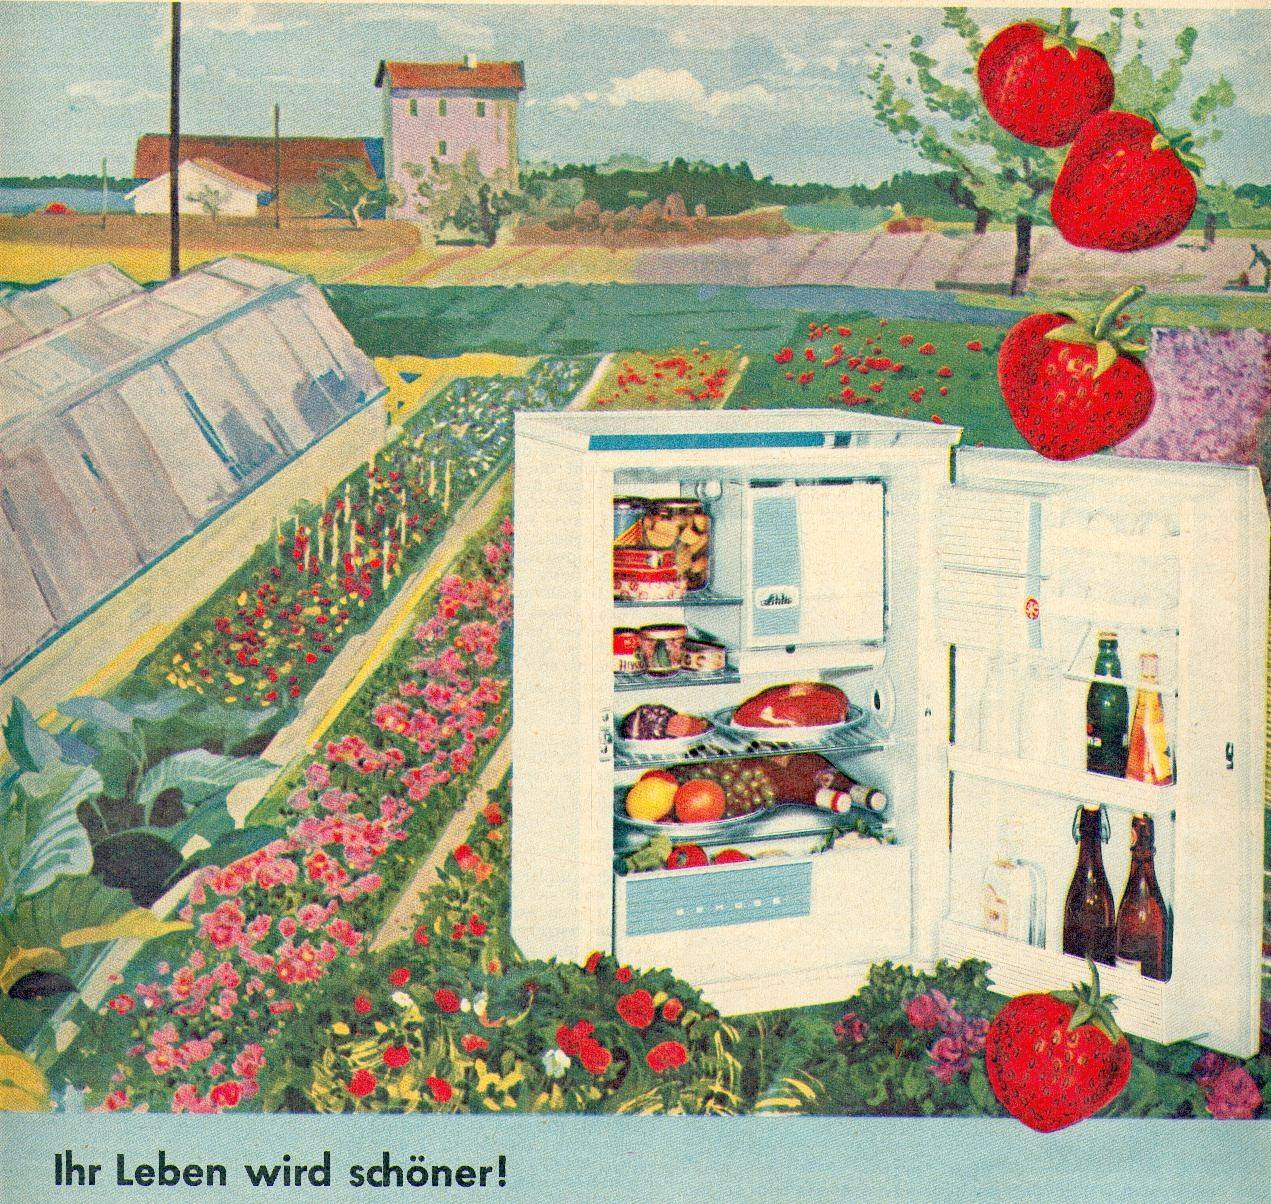
\includegraphics[width=0.73\textwidth]{./History/Spiekermann1.jpg}
    
    \caption{\itshape Cultivation and Civilization: Advertisement of Linde refrigerator, 1959}%\label{fig:profxxx}
   \end{center}
\end{figure}

\begin{}
  \begin{center}
    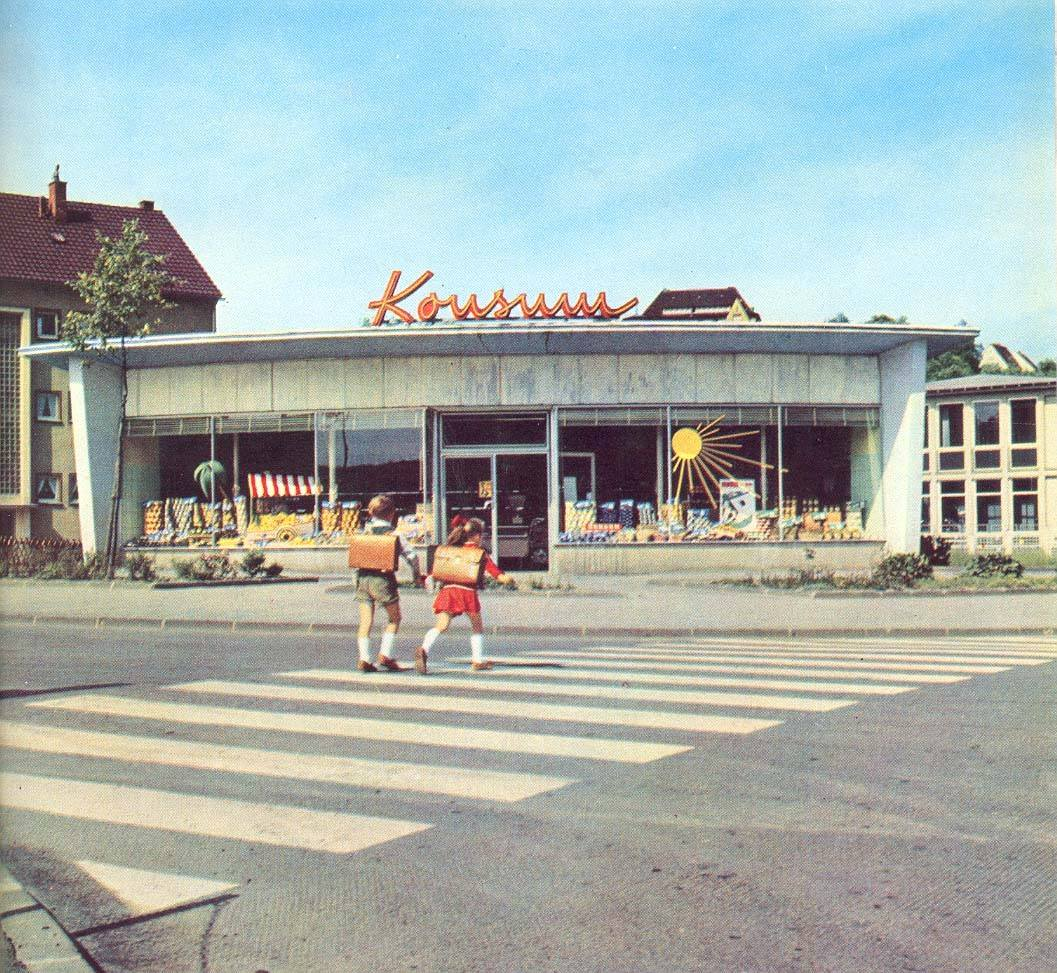
\includegraphics[width=0.72\textwidth]{./History/Spiekermann2.jpg}
    
    \caption{\itshape On the way to a unknown world of affluence, Dortmund 1959}%\label{fig:profxxx}
   \end{center}
\end{figure}

\vspace{0.3cm}
In addition to this project Uwe Spiekermann continued work in his main research areas, mainly in the fields of marketing and retailing. Additionally he arranged (together with two colleagues) a conference on the \textit{History of beer consumption and marketing in $19^{\rm th}$ and $20^{\rm th}$ century}, sponsored by the Gesellschaft f\"{u}r Westf\"{a}lische Wirtschaftsgeschichte, which will take place in Dortmund in June 2007.

\vspace{0.6cm}


\textbf{Funded Projects}\\[-0.25cm]
\begin{enumerate}
\item[$\bullet$]   Scholarship of the Deutsche Forschungsgemeinschaft for the Project \textit{K\"{u}nstliche Kost. Die Durchsetzung der Wissensgesellschaft und die Erfindung der modernen Ern�hrung in Deutschland 1880-2000} (01/2006; 06/2006ff.)
\end{enumerate}



\vspace{0.6cm}
\textbf{Other Professional Activities}\\[-0.25cm]
\begin{enumerate}
\item[$\bullet$] Editorial Committee of "Food and Foodways" (Taylor \& Francis)
\item[$\bullet$] Steering group of the "New Nutrition Science Project" (Global network, supported by the International Union of Nutritionists)
\item[$\bullet$] Scientific advisory board of "Ern\"{a}hrung im Fokus" (Aid)
\item[$\bullet$] Scientific advisory board of "OSSENA - Ern\"{a}hrungsqualit\"{a}t als Lebensqualit\"{a}t" (Research project, financed by the Federal Ministry of Education and Research)
\item[$\bullet$] Scientific Jury of the "F\"{o}rderpreis Ern\"{a}hrungskultur", sponsored by the Johannes Fehr GmbH \& Co. KG
\item[$\bullet$] Visiting lecturer at the University of Vienna, Department of Nutritional Sciences: Lecture/Seminar "Kulturgeschichte der Ern\"{a}hrung"
\item[$\bullet$] Several Radio-Interviews with NDR, WDR, SWR, MDR, mainly on the history of nutrition and retailing.
\end{enumerate}
